% \documentclass[handout]{beamer}
\documentclass{beamer}

\mode<presentation>
{
  \usetheme{ANLBlue}
  % \usefonttheme[onlymath]{serif}
  % \usetheme{Singapore}
  % \usetheme{Warsaw}
  % \usetheme{Malmoe}
  % \useinnertheme{circles}
  % \useoutertheme{infolines}
  % \useinnertheme{rounded}

  \setbeamercovered{transparent=20}
}

\usepackage[english]{babel}
\usepackage[latin1]{inputenc}
\usepackage{alltt,listings,multirow,ulem,siunitx}
\usepackage[absolute,overlay]{textpos}
\TPGrid{1}{1}
\usepackage{pdfpages}
\usepackage{ulem}
\usepackage{multimedia}
\usepackage{multicol}
\newcommand\hmmax{0}
\newcommand\bmmax{0}
\usepackage{bm}
\usepackage{comment}
\usepackage{subcaption}

% font definitions, try \usepackage{ae} instead of the following
% three lines if you don't like this look
\usepackage{mathptmx}
\usepackage[scaled=.90]{helvet}
% \usepackage{courier}
\usepackage[T1]{fontenc}
\usepackage{tikz}
\usetikzlibrary{decorations.pathreplacing}
\usetikzlibrary{shadows,arrows,shapes.misc,shapes.arrows,shapes.multipart,arrows,decorations.pathmorphing,backgrounds,positioning,fit,petri,calc,shadows,chains,matrix}

\newcommand\vvec{\bm v}
\newcommand\bvec{\bm b}
\newcommand\bxk{\bvec_0 \times \kappa_0 \cdot \nabla}
\newcommand\delp{\nabla_\perp}

% \usepackage{pgfpages}
% \pgfpagesuselayout{4 on 1}[a4paper,landscape,border shrink=5mm]

\usepackage{JedMacros}

\newcommand{\timeR}{t_{\mathrm{R}}}
\newcommand{\timeW}{t_{\mathrm{W}}}
\newcommand{\mglevel}{\ensuremath{\ell}}
\newcommand{\mglevelcp}{\ensuremath{\mglevel_{\mathrm{cp}}}}
\newcommand{\mglevelcoarse}{\ensuremath{\mglevel_{\mathrm{coarse}}}}
\newcommand{\mglevelfine}{\ensuremath{\mglevel_{\mathrm{fine}}}}

%solution and residual
\newcommand{\vx}{\ensuremath{x}}
\newcommand{\vc}{\ensuremath{\hat{x}}}
\newcommand{\vr}{\ensuremath{r}}
\newcommand{\vb}{\ensuremath{b}}

%operators
\newcommand{\vA}{\ensuremath{A}}
\newcommand{\vP}{\ensuremath{I_H^h}}
\newcommand{\vS}{\ensuremath{S}}
\newcommand{\vR}{\ensuremath{I_h^H}}
\newcommand{\vI}{\ensuremath{\hat I_h^H}}
\newcommand{\vV}{\ensuremath{\mathbf{V}}}
\newcommand{\vF}{\ensuremath{F}}
\newcommand{\vtau}{\ensuremath{\mathbf{\tau}}}


\title{On reducing communication and improving adaptivity in nonlinear multigrid methods}
\author{{\bf Jed Brown} \texttt{jedbrown@mcs.anl.gov} (ANL and CU Boulder) \\
  \quad Mark Adams (LBL), Matt Knepley (UChicago)
}

% - Use the \inst command only if there are several affiliations.
% - Keep it simple, no one is interested in your street address.
% \institute
% {
%   Mathematics and Computer Science Division \\ Argonne National Laboratory
% }

\date{CU Boulder Applied Math Colloquium, 2014-10-03 \\[1em]
This talk: \url{http://59A2.org/files/20141003-CUBoulder.pdf}}

% This is only inserted into the PDF information catalog. Can be left
% out.
\subject{Talks}


% If you have a file called "university-logo-filename.xxx", where xxx
% is a graphic format that can be processed by latex or pdflatex,
% resp., then you can add a logo as follows:

% \pgfdeclareimage[height=0.5cm]{university-logo}{university-logo-filename}
% \logo{\pgfuseimage{university-logo}}



% Delete this, if you do not want the table of contents to pop up at
% the beginning of each subsection:
% \AtBeginSubsection[]
% {
% \begin{frame}<beamer>
%   \frametitle{Outline}
%   \tableofcontents[currentsection,currentsubsection]
% \end{frame}
% }

% \AtBeginSection[]
% {
%   \begin{frame}<beamer>
%     \frametitle{Outline}
%     \tableofcontents[currentsection]
%   \end{frame}
% }

% If you wish to uncover everything in a step-wise fashion, uncomment
% the following command:

% \beamerdefaultoverlayspecification{<+->}

\begin{document}
\lstset{language=C}
\normalem

\begin{frame}
  \titlepage
\end{frame}

\begin{frame}{Plan: ruthlessly eliminate communication}
  \begin{itemize}
  \item Eliminate, not ``aggregate and amortize''
  \end{itemize}
  \begin{block}{Why?}
    \begin{itemize}
    \item Enables pruning unnecessary work
    \item More scope for dynamic load balance
    \item Tolerance for high-frequency load imbalance
      \begin{itemize}
      \item From irregular computation or hardware error correction
      \end{itemize}
    \item Local recovery despite global coupling
    \end{itemize}
  \end{block}
  \begin{block}{Requirements}
    \begin{itemize}
    \item Must retain optimal convergence with good constants
    \item Flexible, robust, and debuggable
    \end{itemize}
  \end{block}
\end{frame}

\section{$\tau$-adaptivity and multigrid compression}
\begin{frame}[fragile]{Multigrid Preliminaries}
  \begin{figure}
    \centering
    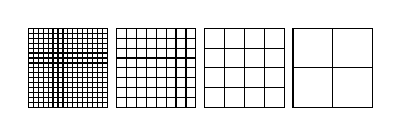
\begin{tikzpicture}
      [>=stealth,
      every node/.style={inner sep=2pt},
      restrict/.style={thick},
      prolong/.style={thick},
      mglevel/.style={rounded rectangle,draw=blue!50!black,fill=blue!20,thick,minimum size=4mm},
      ]
      \begin{scope}\scriptsize
        \newcommand\mgdx{4.0em}
        \newcommand\mgdy{4.0em}
        \newcommand\mgl[1]{(pow(2,#1+1))}
        \newcommand\mgloc[4]{(#1 + #4*\mgdx*#3,#2 + \mgdy*#3)}

        \newcommand\mghx{0.9*\mgdx}
        \newcommand\mghy{0.9*\mgdy}

        \draw[shift=\mgloc{0*\mgdx}{0}{0}{0},
        xstep=\mghy/\mgl{3},
        ystep=\mghy/\mgl{3}]
        (-0.5*\mghy,-0.5*\mghy) grid (0.5*\mghy,0.5*\mghy);

        \draw[shift=\mgloc{1*\mgdx}{0}{0}{0},
        xstep=\mghy/\mgl{2},
        ystep=\mghy/\mgl{2}]
        (-0.5*\mghy,-0.5*\mghy) grid (0.5*\mghy,0.5*\mghy);

        \draw[shift=\mgloc{2*\mgdx}{0}{0}{0},
        xstep=\mghy/\mgl{1},
        ystep=\mghy/\mgl{1}]
        (-0.5*\mghy,-0.5*\mghy) grid (0.5*\mghy,0.5*\mghy);


        \draw[shift=\mgloc{3*\mgdx}{0}{0}{0},
        xstep=\mghy/\mgl{0},
        ystep=\mghy/\mgl{0}]
        (-0.5*\mghy,-0.5*\mghy) grid (0.5*\mghy,0.5*\mghy);
      \end{scope}
    \end{tikzpicture}
    \label{fig:levels}
  \end{figure}
  \textbf{Multigrid} is an $O(n)$ method for solving algebraic problems by defining a hierarchy of scale.
  A multigrid method is constructed from:
  \begin{enumerate}
  \item a sequence of discretizations
    \begin{itemize}
    \item coarser approximations of problem, same or different equations
    \item constructed algebraically or geometrically
    \end{itemize}
  \item intergrid transfer operators
    \begin{itemize}
    \item residual restriction $I_h^H$ (fine to coarse)
    \item state restriction $\hat I_h^H$ (fine to coarse)
    \item partial state interpolation $I_H^h$ (coarse to fine, `prolongation')
    \item state reconstruction $\mathbb{I}_H^h$ (coarse to fine)
    \end{itemize}
  \item Smoothers ($S$)
    \begin{itemize}
    \item correct the high frequency error components
    \item Richardson, Jacobi, Gauss-Seidel, etc.
    \item Gauss-Seidel-Newton or optimization methods
    \item Compatible Monte Carlo, \ldots
    \end{itemize}
  \end{enumerate}
\end{frame}
\begin{frame}{$\tau$ formulation of Full Approximation Scheme (FAS)}
  \begin{itemize}
  \item classical formulation: ``coarse grid \emph{accelerates} fine grid $\searrow \nearrow$
  \item $\tau$ formulation: ``fine grid feeds back into coarse grid'' $\nearrow \searrow$
  \item To solve $N u = f$, recursively apply
    \begin{equation*}
      \begin{split}
        \text{pre-smooth} \:\: & \quad \tilde u^h \gets S^h_{\text{pre}}(u^h_0, f^h) \\
        \text{solve coarse problem for $u^H$} \:\: & \quad N^H u^H = \underbrace{I_h^H f^h}_{f^H} + \underbrace{N^H \hat I_h^H \tilde u^h - I_h^H N^h \tilde u^h}_{\tau_h^H} \\
        \text{correction and post-smooth} \:\: & \quad u^h \gets S^h_{\text{post}} \Big( \tilde u^h + I_H^h (u^H - \hat I_h^H \tilde u^h), f^h \Big) \\
      \end{split}
    \end{equation*}
    \begin{tabular}{llll}
      \toprule
      $I_h^H$ & residual restriction & $\hat I_h^H$ & solution restriction \\
      $I_H^h$ & solution interpolation & $f^H = I_h^H f^h$ & restricted forcing \\
      $\{S^h_{\text{pre}},S^h_{\text{post}}\}$ & \multicolumn{3}{l}{smoothing operations on the fine grid} \\
      \bottomrule
    \end{tabular}
  \item At convergence, $u^{H*} = \hat I_h^H u^{h*}$ solves the $\tau$-corrected coarse grid equation
    $N^H u^H = f^H + \tau_h^H$,
    thus $\tau_h^H$ is the ``fine grid feedback'' that makes the coarse grid equation accurate.
  \item $\tau_h^H$ is \emph{local} and need only be recomputed where it becomes stale.
  \item Interpretation by Achi Brandt in 1977, many tricks followed
  \end{itemize}
\end{frame}


\begin{frame}{Model problem: $\pfrak$-Laplacian with slip boundary conditions}
  \begin{itemize}
  \item 2-dimensional model problem for power-law fluid cross-section
    \begin{equation*}
      -\div \big(\abs{\nabla u}^{\pfrak-2} \nabla u \big) - f = 0, \qquad 1 \le \pfrak \le \infty
    \end{equation*}
    Singular or degenerate when $\nabla u = 0$
  \item Regularized variant
    \begin{gather*}
      -\div (\eta \nabla u) - f = 0 \\
      \eta(\gamma) = (\epsilon^2 + \gamma)^{\frac{\pfrak-2}{2}} \qquad \gamma(u) = \half \abs{\nabla u}^2
    \end{gather*}
  \item Friction boundary condition on one side of domain
    \begin{gather*}
      \nabla u \cdot \bm n + A(x) \abs{u}^{q-1} u = 0
    \end{gather*}
  \end{itemize}
\end{frame}

\begin{frame}{Model problem: $\pfrak$-Laplacian with slip boundary conditions}
  \begin{itemize}
  \item $\pfrak = 1.3$ and $q = 0.2$, checkerboard coefficients $\{10^{-2},1\}$
  \item Friction coefficient $A=0$ in center, 1 at corners
  \end{itemize}
  \begin{columns}
    \begin{column}{0.5\textwidth}
      \only<1>{\includegraphics[width=\textwidth]{figures/MG/ex15-friction/visit0010.png}}
      \only<2>{\includegraphics[width=\textwidth]{figures/MG/ex15-friction/visit0011.png}}
      \only<3>{\includegraphics[width=\textwidth]{figures/MG/ex15-friction/visit0012.png}}
      \only<4>{\includegraphics[width=\textwidth]{figures/MG/ex15-friction/visit0013.png}}
      \only<5>{\includegraphics[width=\textwidth]{figures/MG/ex15-friction/visit0014.png}}
      \only<6>{\includegraphics[width=\textwidth]{figures/MG/ex15-friction/visit0015.png}}
    \end{column}
    \begin{column}{0.5\textwidth}
      \includegraphics[width=\textwidth]{figures/MG/newton-convergence.png}
    \end{column}
  \end{columns}
\end{frame}

\begin{frame}{$\tau$ corrections}
  \begin{figure}
  \centering
  \begin{subfigure}[b]{0.18\textwidth}
    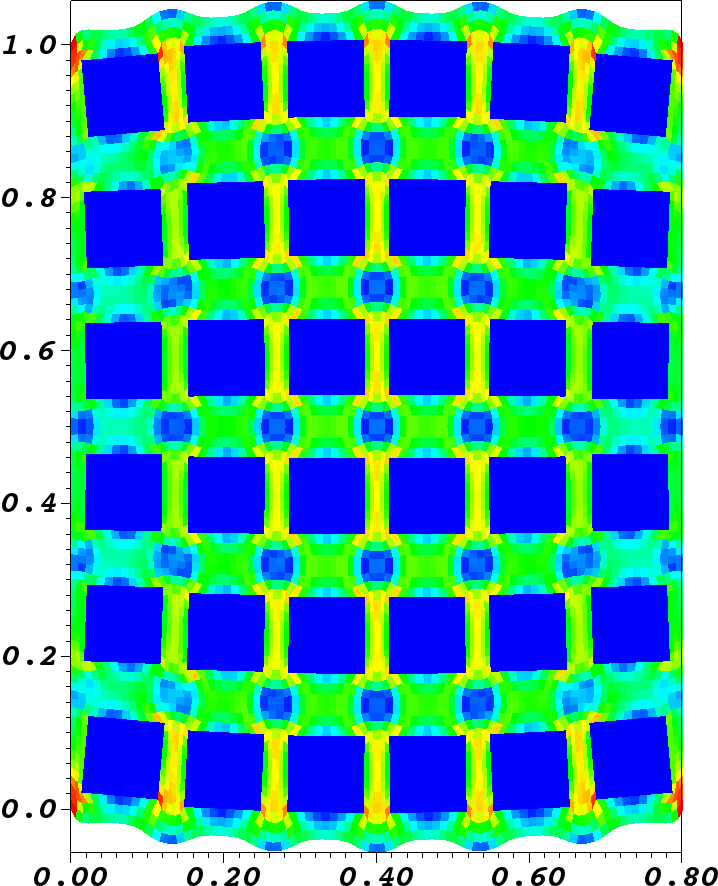
\includegraphics[width=\textwidth]{figures/MG/ElasticityCompressTrim}
    %\caption{Initial solution.}\label{fig:elast-initial}
  \end{subfigure} ~
  \begin{subfigure}[b]{0.18\textwidth}
    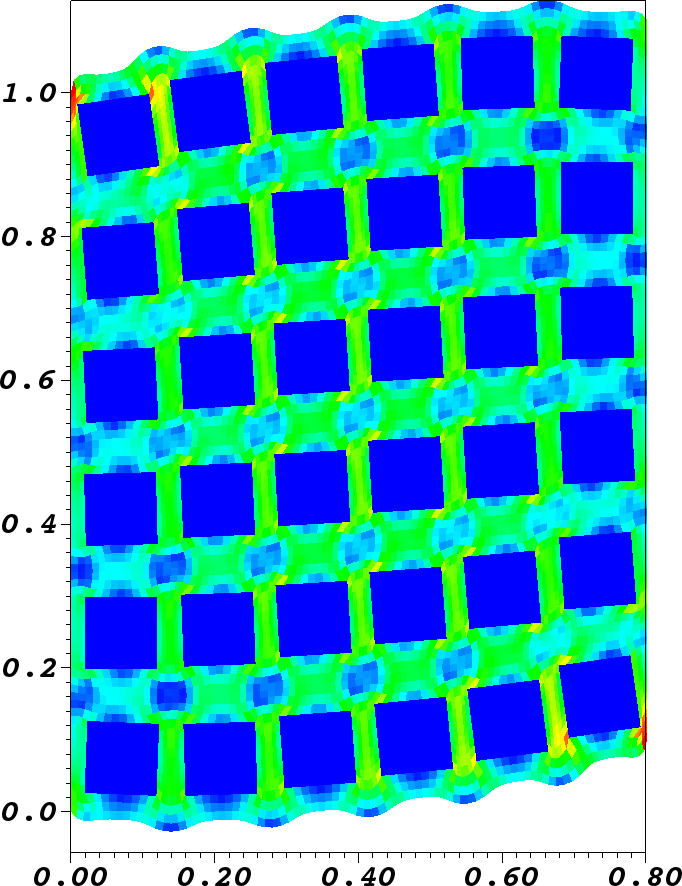
\includegraphics[width=\textwidth]{figures/MG/ElasticityCompressShearTrim}
    %\caption{Increment.}\label{fig:elast-increment}
  \end{subfigure} ~
  \begin{subfigure}[b]{0.28\textwidth}
    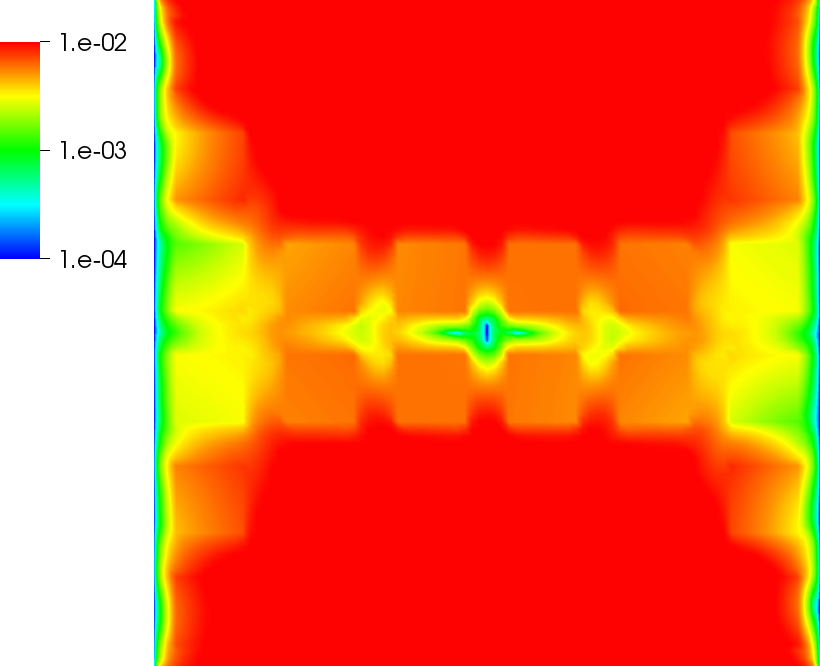
\includegraphics[width=\textwidth]{figures/MG/ElasticityCompressErrorNoTauTrim}
    %\caption{Smoothed error without $\tau$.}\label{fig:elast-error-notau}
  \end{subfigure} ~
  \begin{subfigure}[b]{0.28\textwidth}
    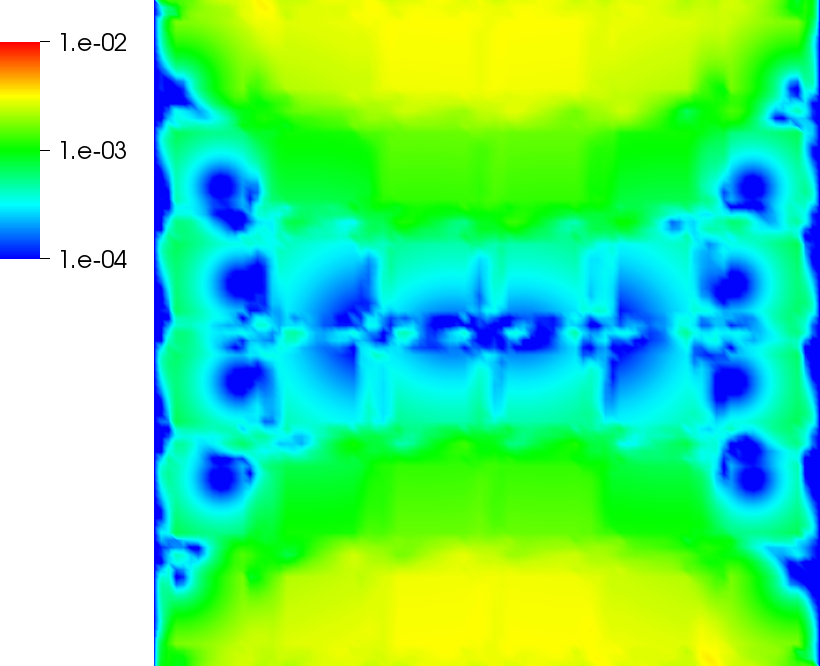
\includegraphics[width=\textwidth]{figures/MG/ElasticityCompressErrorTauTrim}
    %\caption{Smoothed error with $\tau$.}\label{fig:elast-error-tau}
  \end{subfigure}
  \begin{itemize}
  \item Plane strain elasticity, $E=1000,\nu=0.4$ inclusions in $E=1,\nu=0.2$ material, coarsen by $3^2$.
  \item Solve initial problem everywhere and compute $\tau_h^H = A^H \hat I_h^H u^h - I_h^H A^h u^h$
  \item Change boundary conditions and solve FAS coarse problem
    \begin{equation*}
      N^H \acute u^H = \underbrace{I_h^H \acute f^h}_{\acute f^H} + \underbrace{N^H \hat I_h^H \tilde u^h - I_h^H N^h \tilde u^h}_{\tau_h^H}
    \end{equation*}
  \item Prolong, post-smooth, compute error $e^h = \acute u^h - (N^h)^{-1} \acute f^h$
  \item<2> \alert{Coarse grid \emph{with $\tau$} is nearly $10\times$ better accuracy}
  \end{itemize}
  % \caption{Plane strain elasticity, $E=1000,\nu=0.4$ inclusions in $E=1,\nu=0.2$ material.  2-level multigrid with coarsening factor of $3^2$.
  %   Panes (a) and (b) show the deformed body colored by strain.
  %   The initial problem of compression by 0.2 from the right is solved (a) and $\tau = A^H \hat I_h^H u^h - I_h^H A^h u^h$ is computed.
  %   Then a shear increment of 0.1 in the $y$ direction is added to the boundary condition, and the coarse-level problem is resolved, interpolated to the fine-grid, and a post-smoother is applied.
  %   When the coarse problem is solved without a $\tau$ correction (c), the displacement error is nearly $10\times$ larger than when $\tau$ is included in the right hand side of the coarse problem (d).
  % }\label{fig:tau-valid}
  % ./ex49 -mx 90 -my 90 -da_refine_x 3 -da_refine_y 3 -elas_ksp_converged_reason -elas_ksp_rtol 1e-8 -no_view -c_str 3 -sponge_E0 1 -sponge_E1 1e3 -sponge_nu0 0.4 -sponge_nu1 0.2 -sponge_t 3 -sponge_w 9 -u_o vtk:ex49_sol.vts -use_nonsymbc -elas_pc_type mg -elas_pc_mg_levels 2 -elas_pc_mg_galerkin -tau1_o vtk:ex49_tau1.vts -tau2_o vtk:ex49_tau2.vts -taudiff_o vtk:ex49_taudiff.vts -u2_o vtk:ex49_sol2.vts -u2c_o vtk:ex49_sol2c.vts -u3_o vtk:ex49_sol3.vts -u4_o vtk:ex49_sol4.vts -u2err_o vtk:ex49_sol2err.vts -u3err_o vtk:ex49_sol3err.vts -u3c_o vtk:ex49_sol3c.vts -tau3_o vtk:ex49_tau3.vts
\end{figure}
\end{frame}

\begin{frame}{$\tau$ adaptivity: an idea for heterogeneous media}
  \begin{itemize}
  \item Applications with localized nonlinearities
    \begin{itemize}
    \item Subduction, rifting, rupture/fault dynamics
    \item Carbon fiber, biological tissues, fracture
    \end{itemize}
  \item Adaptive methods fail for heterogeneous media
    \begin{itemize}
    \item Rocks are rough, solutions are not ``smooth''
    \item Cannot build accurate coarse space without scale separation
    \end{itemize}
  \item $\tau$ adaptivity
    \begin{itemize}
    \item Fine-grid work needed everywhere at first
    \item Then $\tau$ becomes accurate in nearly-linear regions
    \item Only visit fine grids in ``interesting'' places: active nonlinearity, drastic change of solution
    \end{itemize}
  \end{itemize}
\end{frame}

\begin{frame}{Comparison to nonlinear domain decomposition}
  \begin{itemize}
  \item ASPIN (Additive Schwarz preconditioned inexact Newton) \\
    \begin{itemize}
    \item Cai and Keyes (2003)
    \item More local iterations in strongly nonlinear regions
    \item Each nonlinear iteration only propagates information locally
    \item Many real nonlinearities are activated by long-range forces
      \begin{itemize}
      \item locking in granular media (gravel, granola)
      \item binding in steel fittings, crack propagation
      \end{itemize}
    \item Two-stage algorithm has different load balancing
      \begin{itemize}
      \item Nonlinear subdomain solves
      \item Global linear solve
      \end{itemize}
    \end{itemize}
  \item $\tau$ adaptivity
    \begin{itemize}
    \item Minimum effort to communicate long-range information
    \item Nonlinearity sees effects as accurate as with global fine-grid feedback
    \item Fine-grid work always proportional to ``interesting'' changes
    \end{itemize}
  \end{itemize}
\end{frame}

\begin{frame}{Nonlinear and matrix-free smoothing}
  \begin{itemize}
  \item matrix-based smoothers require global linearization
  \item nonlinearity often more efficiently resolved locally
  \item nonlinear additive or multiplicative Schwarz
  \item nonlinear/matrix-free is good if
    \[ C = \frac{(\text{cost to evaluate residual at one point}) \cdot N}{(\text{cost of global residual})} \sim 1 \]
    \begin{itemize}
    \item finite difference: $C < 2$
    \item finite volume: $C \sim 2$, depends on reconstruction
    \item finite element: $C \sim \text{number of vertices per cell}$
    \end{itemize}
  \item larger block smoothers help reduce $C$
  \item additive correction like Jacobi reduces $C$, \\
    but need to assemble corrector/scaling
  \end{itemize}
  \vspace{-4.5em}
  \hfill \includegraphics[width=0.3\textwidth]{figures/NodeStencil}
\end{frame}


\subsection{Reducing communication and memory bandwidth}
\begin{frame}{Low communication MG}
  \begin{columns}
    \begin{column}{0.55\textwidth}
      \begin{itemize}
      \item {\color{red} red arrows} can be removed by $\tau$-FAS with overlap
      \item {\color{blue} blue arrows} can also be removed, but then
        algebraic convergence stalls when discretization error is
        reached
      \item no simple way to check that discretization error is obtained
      \item if fine grid state is not stored, use compatible relaxation to complete prolongation $P$
      \item ``Segmental refinement'' by Achi Brandt (1977)
      \item 2-process case by Brandt and Diskin (1994)
      \end{itemize}
    \end{column}
    \begin{column}{0.45\textwidth}
      \vspace{-2em}
      \includegraphics[width=\textwidth]{figures/MG/LowCommunication}
    \end{column}
  \end{columns}
\end{frame}

\begin{frame}{Segmental refinement: no horizontal communication}
  \begin{itemize}
  \item 27-point second-order stencil, manufactured analytic solution
  \item 5 SR levels: $16^3$ cells/process local coarse grid
  \item $\text{Overlap} = \text{Base} + (L-\ell) \text{Increment}$
    \begin{itemize}
    \item Implementation requires even number of cells---round down.
    \end{itemize}
  \item FMG with $V(2,2)$ cycles
  \end{itemize}
  \begin{columns}
    \begin{column}{0.4\textwidth}
      \begin{table}\small
        \centering\caption{$\norm{e_{SR}}_\infty / \norm{e_{FMG}}_\infty$}\label{tab:sr-error}
        \begin{tabular}{l rrr}
          \toprule
          & \multicolumn{3}{c}{Base} \\
          Increment & 1 & 2 & 3 \\
          \midrule
          1 & {\color{red} 1.59} & {\color{red} 2.34} & 1.00 \\
          2 & 1.00 & 1.00 & 1.00 \\
          3 & 1.00 & 1.00 & 1.00 \\
          \bottomrule
        \end{tabular}
      \end{table}
    \end{column}
    \begin{column}{0.6\textwidth}
      \includegraphics[width=\textwidth]{figures/MG/weak_scaling_edison-eps-converted-to.pdf}
    \end{column}
  \end{columns}
\end{frame}

\begin{frame}{Reducing memory bandwidth}
  \includegraphics[width=\textwidth]{figures/MG/SRMGWindow}
  \begin{itemize}
  \item Sweep through ``coarse'' grid with moving window
  \item Zoom in on new slab, construct fine grid ``window'' in-cache
  \item Interpolate to new fine grid, apply pipelined smoother ($s$-step)
  \item Compute residual, accumulate restriction of state and residual into coarse grid, expire slab from window
  \end{itemize}
\end{frame}

\begin{frame}{Arithmetic intensity of sweeping visit}
  \begin{itemize}
  \item Assume 3D cell-centered, 7-point stencil
  \item 14 flops/cell for second order interpolation
  \item $\ge 15$ flops/cell for fine-grid residual or point smoother
  \item 2 flops/cell to enforce coarse-grid compatibility
  \item 2 flops/cell for plane restriction
  \item assume coarse grid points are reused in cache
  \item Fused visit reads $u^H$ and writes $\hat I_h^H u^h$ and $I_h^H r^h$
  \item Arithmetic Intensity
    \begin{equation}
      \frac{{\overbrace{15}^{\text{interp}}} + {\overbrace{2\cdot (15+2)}^{\text{compatible relaxation}}} + \overbrace{2\cdot 15}^{\text{smooth}} + \overbrace{15}^{\text{residual}} + \overbrace{2}^{\text{restrict}}}{3 \cdot \texttt{sizeof(scalar)} / \underbrace{2^3}_{\text{coarsening}}} \gtrsim 30
    \end{equation}
  \item Still $\gtrsim 10$ with non-compressible fine-grid forcing
  \end{itemize}
\end{frame}

\begin{frame}{Regularity}
  Accuracy of recovery depends on operator regularity
  \begin{itemize}
  \item Even with regularity, we can only converge up to discretization error, unless we add a \emph{consistent} fine-grid residual evaluation
  \item Visit fine grid with some overlap, but patches do not agree exactly in overlap
  \item Need decay length for high-frequency error components (those that restrict to zero) that is bounded with respect to grid size
  \item Required overlap $J$ is proportional to the number of cells to cover decay length
  \item Can enrich coarse space along boundary, but causes loss of coarse-grid sparsity
  \item Brandt and Diskin (1994) has two-grid LFA showing $J \lesssim 2$ is sufficient for Laplacian
  \item With $L$ levels, overlap $J(k)$ on level $k$,
    \begin{equation*}
      2J(k) \ge s (L-k+1)
    \end{equation*}
    where $s$ is the smoothness order of the solution or the discretization order (whichever is smaller)
  \end{itemize}
\end{frame}

\begin{frame}{Basic resilience strategy}
  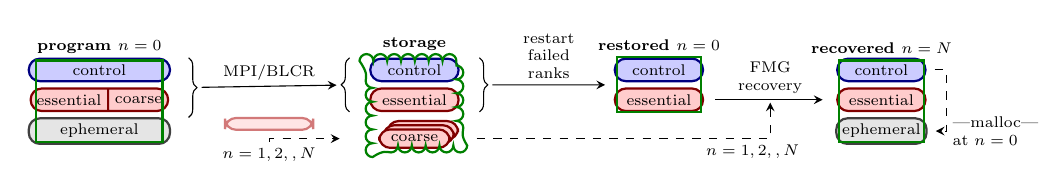
\begin{tikzpicture}
    [scale=0.8,every node/.style={scale=0.8},
    >=stealth,
    control/.style={rectangle,rounded corners,draw=blue!50!black,fill=blue!20,thick,minimum width=5em},
    essential/.style={rectangle,rounded corners,draw=red!50!black,fill=red!20,thick,minimum width=5em},
    ephemeral/.style={rectangle,rounded corners,draw=gray!50!black,fill=gray!20,thick,minimum width=5em},
    statebox/.style={rectangle,draw=green!50!black,thick},
    statetitle/.style={rectangle,draw=green!50!black,fill=green!20,thick},
    storebox/.style={rectangle,draw=},
    rightbrace/.style={decorate,decoration={brace,amplitude=1ex,raise=4pt}},
    leftbrace/.style={decorate,decoration={brace,amplitude=1ex,raise=4pt,mirror}}
    ]
    \scriptsize
    \node[control,minimum width=8em] (progcontrol) {control};
    \node[essential,below=2pt of progcontrol.south,rectangle split,rectangle split parts=2,rectangle split horizontal,minimum width=12em] (progessential) {essential \nodepart{two} coarse};
    \node[ephemeral,minimum width=8em,below=2pt of progessential.south] (progephemeral) {ephemeral};
    \node[statebox,fit=(progcontrol)(progessential)(progephemeral)] (progbox) {};
    \node[above=0pt of progbox.north,anchor=south] {\textbf{program $n=0$}};

    \node[control,right=9em of progcontrol] (storecontrol) {control};
    \node[essential,below=2pt of storecontrol.south] (storeessential) {essential};
    \node[essential,minimum width=4em,below=6pt of storeessential.south, double copy shadow] (storecoarse) {coarse};
    \node[statebox,decorate,decoration={bumps,mirror},fit=(storecontrol)(storecoarse)] (storebox) {};
    \node[above=1pt of storebox.north,anchor=south] {\textbf{storage}};

    \node[control,right=7em of storecontrol] (reccontrol) {control};
    \node[essential,below=2pt of reccontrol.south] (recessential) {essential};
    \node[statebox,fit=(reccontrol)(recessential)] (recbox) {};
    \node[above=0pt of recbox.north,anchor=south] {\textbf{restored $n=0$}};

    \node[control,right=6em of reccontrol] (donecontrol) {control};
    \node[essential,below=2pt of donecontrol.south] (doneessential) {essential};
    \node[ephemeral,below=2pt of doneessential.south] (doneephemeral) {ephemeral};
    \node[statebox,fit=(donecontrol)(doneephemeral)] (donebox) {};
    \node[above=0pt of donebox.north,anchor=south] {\textbf{recovered $n=N$}};

    \draw[decorate,decoration={brace,amplitude=1ex,raise=4pt}] ($(progcontrol.north east) + (3pt,0)$) -- ($(progephemeral.north east) + (3pt,0)$) node[midway,xshift=1ex] (progbrace) {};
    \draw[leftbrace] ($(storecontrol.north west) - (4pt,0)$) -- ($(storeessential.south west) - (4pt,0)$) node[midway,xshift=-1ex] (storebrace) {};
    \draw[rightbrace] ($(storecontrol.north east) + (4pt,0)$) -- ($(storeessential.south east) + (4pt,0)$) node[midway,xshift=1ex] (storerbrace) {};
    \draw[->,shorten >=4pt,shorten <=4pt] (progbrace) -- (storebrace) node[midway,above] (midarrow) {MPI/BLCR};

    \node[below=1.4em of midarrow,essential,draw=red!50!gray!70,fill=red!10] (coarserun) {};
    \draw[->,dashed,shorten >=14pt,shorten <=4pt] (coarserun) |- (storecoarse) node [near start,below,yshift=-3pt] {\scriptsize $n=1,2,\dotsc,N$};
    \draw[->,shorten >=4pt,shorten <=4pt] (storerbrace) -- (recbox.west) node[midway,above,text width=5em,align=center] (midarrow) {restart failed ranks};
    \draw[->,shorten >=5pt,shorten <=4pt] (recessential.east) -- (doneessential) node[midway,above,text width=5em,align=center] (fmgrecover) {FMG recovery};
    \draw[->,dashed,shorten >=1pt,shorten <=3pt] ($(storecoarse.east) + (1em,0)$) -| (fmgrecover) node[midway,below,xshift=-1em] {\scriptsize $n=1,2,\dotsc,N$};
    \draw[->,dashed,shorten >=3pt,shorten <=3pt] (donecontrol.east) -| ($(donecontrol.east) + (3ex,0)$) |- (doneephemeral.east) node[midway,right,text width=4em] {\cverb|malloc| at $n=0$};
  \end{tikzpicture}
\begin{description}
\item[control] contains program stack, solver configuration, etc.
\item[essential] program state that cannot be easily reconstructed: time-dependent solution, current optimization/bifurcation iterate
\item[ephemeral] easily recovered structures: assembled matrices, preconditioners, residuals, Runge-Kutta stage solutions
\end{description}
\begin{itemize}
\item Essential state at time/optimization step $n$ is \alert{inherently globally coupled} to step $n-1$ (otherwise we could use an explicit method)
\item \emph{Coarse} level checkpoints are orders of magnitude smaller, but allow rapid recovery of essential state
\item FMG recovery needs only \alert{nearest neighbors}
\end{itemize}
\end{frame}

\begin{frame}[fragile]{Multiscale compression and recovery using $\tau$ form}
   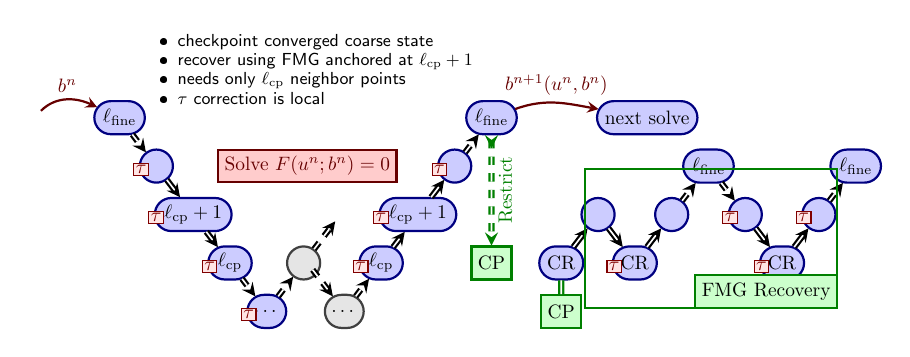
\begin{tikzpicture}
    [scale=0.7,every node/.style={scale=0.7},
    >=stealth,
    restrict/.style={thick,double},
    prolong/.style={thick,double},
    cprestrict/.style={green!50!black,thick,double,dashed},
    control/.style={rectangle,red!40!black,draw=red!40!black,thick},
    mglevel/.style={rounded rectangle,draw=blue!50!black,fill=blue!20,thick,minimum size=6mm},
    checkpoint/.style={rectangle,draw=green!50!black,fill=green!20,thick,minimum size=6mm},
    mglevelhide/.style={rounded rectangle,draw=gray!50!black,fill=gray!20,thick,minimum size=6mm},
    tau/.style={text=red!50!black,draw=red!50!black,fill=red!10,inner sep=1pt},
    crelax/.style={text=green!50!black,fill=green!10,inner sep=0pt}
    ]
    \begin{scope}
      \newcommand\mgdx{1.9em}
      \newcommand\mgdy{2.5em}
      \newcommand\mgloc[4]{(#1 + #4*\mgdx*#3,#2 + \mgdy*#3)}
      \node[mglevel] (fine0) at \mgloc{0}{0}{4}{-1} {\mglevelfine};
      \node[mglevel] (finem1down0) at \mgloc{0}{0}{3}{-1} {};
      \node[mglevel] (cp1down0) at \mgloc{0}{0}{2}{-1} {$\mglevelcp+1$};
      \node[mglevel] (cpdown0) at \mgloc{0}{0}{1}{-1} {\mglevelcp};
      \node[mglevel] (coarser0) at \mgloc{0}{0}{0}{0} {\ldots};

      \node[mglevelhide] (cpup0) at \mgloc{0}{0}{1}{1} {};
      \node (cp1up0) at \mgloc{0}{0}{2}{1} {};

      \node (cpdown1) at \mgloc{4em}{0}{1}{-1} {};
      \node[mglevelhide] (coarser1) at \mgloc{4em}{0}{0}{1} {\ldots};
      \node[mglevel] (cpup1) at \mgloc{4em}{0}{1}{1} {\mglevelcp};
      \node[mglevel] (cp1up1) at \mgloc{4em}{0}{2}{1} {$\mglevelcp+1$};
      \node[mglevel] (finem1up1) at \mgloc{4em}{0}{3}{1} {};
      \node[mglevel] (fine1) at \mgloc{4em}{0}{4}{1} {\mglevelfine};

      \draw[->,restrict,dashed] (fine0) -- (finem1down0);
      \draw[->,restrict] (finem1down0) -- (cp1down0);
      \draw[->,restrict] (cp1down0) -- (cpdown0);
      \draw[->,restrict,dashed] (cpdown0) -- (coarser0);
      \draw[->,prolong,dashed] (coarser0) -- (cpup0);
      \draw[->,prolong,dashed] (cpup0) -- (cp1up0);

      \draw[->,restrict,dashed] (cpdown1) -- (coarser1);
      \draw[->,prolong,dashed] (coarser1) -- (cpup1);
      \draw[->,prolong] (cpup1) -- (cp1up1);
      \draw[->,prolong] (cp1up1) -- (finem1up1);
      \draw[->,prolong,dashed] (finem1up1) -- (fine1);

      \node[checkpoint] at (4em + \mgdx*4,\mgdy) (cp) {CP};
      \draw[>->,cprestrict] (fine1) -- node[below,sloped] {Restrict} (cp);

      \node[left=\mgdx of fine0] (bnanchor) {};
      \node[control,fill=red!20] at (1.1*\mgdx,3*\mgdy) {Solve $F(u^n;b^n) = 0$};
      \node[mglevel,right=of fine1] (finedt) {next solve};
      \draw[->, >=stealth, control] (fine1) to[out=20,in=170] node[above] {$b^{n+1}(u^n,b^n)$} (finedt);
      \draw[->, >=stealth, control] (bnanchor) to[out=45,in=155] node[above] {$b^n$} (fine0);

      % Recovery process
      \begin{scope}[xshift=8*\mgdx]
        \node[checkpoint] (rcp) at \mgloc{0}{0}{0}{0} {CP};
        \node[mglevel] (r0a) at \mgloc{0}{\mgdy}{0}{0} {CR};
        \node[mglevel] (r1a) at \mgloc{0}{\mgdy}{1}{1} {};
        \node[mglevel] (r0b) at \mgloc{2*\mgdx}{\mgdy}{0}{0} {CR};
        \node[mglevel] (r1b) at \mgloc{2*\mgdx}{\mgdy}{1}{1} {};
        \node[mglevel] (r2b) at \mgloc{2*\mgdx}{\mgdy}{2}{1} {\mglevelfine};
        \node[mglevel] (r1c) at \mgloc{6*\mgdx}{\mgdy}{1}{-1} {};
        \node[mglevel] (r0d) at \mgloc{6*\mgdx}{\mgdy}{0}{0} {CR};
        \node[mglevel] (r1d) at \mgloc{6*\mgdx}{\mgdy}{1}{1} {};
        \node[mglevel] (r2d) at \mgloc{6*\mgdx}{\mgdy}{2}{1} {\mglevelfine};

        \draw[-,prolong,green!50!black] (rcp) -- (r0a);
        \draw[->,prolong] (r0a) -- (r1a);
        \draw[->,restrict] (r1a) -- (r0b);
        \draw[->,restrict] (r0b) -- (r1b);
        \draw[->,restrict,dashed] (r1b) -- (r2b);
        \draw[->,restrict,dashed] (r2b) -- (r1c);
        \draw[->,restrict] (r1c) -- (r0d);
        \draw[->,restrict] (r0d) -- (r1d);
        \draw[->,restrict,dashed] (r1d) -- (r2d);

        \foreach \smooth in {finem1down0, cp1down0, cpdown0, coarser0,
          cpup1, cp1up1, finem1up1,
          r0b,r1c,r0d,r1d} {
          \node[above left=-5pt of \smooth.west,tau] {$\tau$};
        }
        \node[rectangle,fill=none,draw=green!50!black,thick,fit=(rcp)(r2d)] (recoverbox) {};
        \node[rectangle,draw=green!50!black,fill=green!20,thick,minimum size=6mm,above={0cm of recoverbox.south east},anchor=south east] (recover) {FMG Recovery};
      \end{scope}
      \node (notation) at (\mgdx,5*\mgdy) {
        \begin{minipage}{18em}\small\sf
          \begin{itemize}\addtolength{\itemsep}{-5pt}
          \item checkpoint converged coarse state
          \item recover using FMG anchored at $\mglevelcp+1$
          \item needs only $\mglevelcp$ neighbor points
          \item $\tau$ correction is local
          \end{itemize}
        \end{minipage}
      };
    \end{scope}
  \end{tikzpicture}
  \begin{itemize}
  \item Normal multigrid cycles visit all levels moving from $n \to n+1$
  \item FMG recovery only accesses levels finer than $\ell_{CP}$
  % \item Only failed processes and neighbors participate in recovery
  \item Lightweight checkpointing for transient adjoint computation
  \item Postprocessing applications, e.g., in-situ visualization at high temporal resolution in part of the domain
  \end{itemize}
\end{frame}

\begin{frame}{First-order cost model for FAS resilience}
  Extend first-order locality-unaware model of Young (1974):
  \begin{description}
  \item[$\timeW$] time to write a heavy fine-grid checkpointed state
  \item[$\timeR$] time to read back lost state
  \item[$R$] fraction of forward simulation needed for recomputation from a saved state
  \item[$P$] the heavy checkpoint interval
  \item[$M$] mean time to failure
  \end{description}
  Neglect cost of I/O for lightweight coarse-grid checkpoints
  \begin{equation*}\label{eq:overhead}
    \text{Overhead} = 1 - \text{AppUtilization} = \underbrace{\frac{\timeW}{P}}_{\text{writing}}
    + \underbrace{\frac{\timeR}{M}}_{\text{reading after failure}}
    + \underbrace{\frac{R P}{2M}}_{\text{recomputation}}
  \end{equation*}
  Minimized for a heavy checkpointing interval $P = \sqrt{2 M \timeW / R}$
  \begin{equation*}\label{eq:minoverhead}
    \text{Overhead}^* = \sqrt{2 \timeW R / M} + \timeR / M
    % $ \text{Overhead}^* = \sqrt{\frac{2 \timeW R}{M}} + \frac{\timeR}{M} $,
  \end{equation*}
  where the first term is always larger than the second.
  Conventional checkpointing schemes store only fine-grid state, thus $R=1$ (recovery costs the same as initial computation).
\end{frame}

\begin{frame}{Other uses}
  \begin{itemize}
  \item Transient adjoints
    \begin{itemize}
    \item Adjoint model runs backward-in-time, needs state from solution of forward model
    \item Status quo: hierarchical checkpointing
    \item Memory-constrained and requires computing forward model multiple times
    \item If forward model is stiff, each step has global dependence
    \item Compression via $\tau$-FAS accelerates recomputation, can be local
    \end{itemize}
  \item Visualization and analysis
    \begin{itemize}
    \item Targeted visualization in small part of domain
    \item Interesting features emergent so can't predict where to look
    \end{itemize}
  \end{itemize}
\end{frame}

\begin{frame}{Outlook on $\tau$-FAS adaptivity and compression}
  \begin{itemize}
  \item Benefits of AMR without fine-scale smoothness
  \item Coarse-centric restructuring is a major interface change
  \item Nonlinear smoothers (and discretizations)
    \begin{itemize}
    \item Smooth in neighborhood of ``interesting'' fine-scale features
    \item Which discretizations can provide efficient matrix-free smoothers?
    \item Does there exist an efficient smoother based on element Neumann problems?
    \end{itemize}
  \item Dynamic load balancing
  \item Reliability of error estimates for refreshing $\tau$
    \begin{itemize}
    \item We want a coarse indicator for whether $\tau$ needs to change
    \end{itemize}
  \item Worthwhile for resilience and to better use hardware
  \end{itemize}
\end{frame}

\end{document}
